\documentclass[11pt,titlepage]{article}
\usepackage{pset}

\newcommand*{\X}{\mathfrak{X}}
\newcommand*{\Mod}{\mathcal{M}}
\newcommand*{\vbar}{\;\big\vert\;}
\newcommand*{\mle}{\theta_{\text{mle}}}
\DeclareMathOperator{\Mixt}{Mixt}
\DeclareMathOperator{\Sec}{Sec}
\DeclareMathOperator*{\argmax}{arg\ max}
\newcommand*{\parop}[1]{\frac{\partial}{\partial #1}}

\numberwithin{equation}{section}

\title{The Restricted Boltzmann Machine}
\author{Aaron Pribadi}
\date{November 2011}

\begin{document}

\maketitle

\tableofcontents

\pagebreak

\section{What is Algebraic Statistics?}

    Algebraic statistics is a relatively new field that examines statistical
    questions using algebraic geometry and commutative algebra.  Once a problem
    has been cast in the language of algebra, a number of computational tools
    can be brought to bear.  For example, one of the early papers in the field
    analyzed contingency tables using Monte Carlo algorithms with Gröbner bases.
    \cite{DS98}.

    Algebraic statistics also offers a geometric point of view on families of
    probability distributions; the tendency is toward intrinsically defined
    objects in lieu of explicit coordinate systems.  In this light, algebraic
    statistics might be seen as in the tradition of information geometry, a
    field pioneered in the 1980s that applied the techniques of Riemannian
    geometry to probability models (see for example \cite{Ama}).

    An introduction to the field of algebraic statistics may be found in
    \cite{DSS08} and a brief history of the field may be found in \cite{Ric09}.

    Our goal is to examine a particular statistical model, the \emph{Restricted
    Boltzmann Machine}, from the point of view of algebraic statistics building
    from prior work in that direction, especially \cite{CMS09}.  The Restricted
    Boltzmann Machine has recently become the centerpiece of certain
    developments in the machine learning community, and several basic questions
    remain unanswered.

\section{The Geometry of Statistical Models}
    \subsection{The Probability Simplex}

    We usually consider probability distributions over finite sets.  The space
    of all such distributions corresponds to a geometric object.
    
    \begin{definition} The \emph{probability simplex} of dimension $N$ (also
    called the \emph{standard simplex}) is the space
    \[
        \Delta_N = 
        \left\{(x_1, \ldots, x_{N+1}) \vbar \sum_{i=1}^{N+1} x_i= 1, x_i \ge 0 \right\} 
        \subset
        \R^{N+1}.
    \]
    The subscript $N$ indicates the dimension of the simplex.
    \end{definition}
    A \emph{simplex} in general is the image of a standard simplex under any
    affine transformation.  Low dimensional simplices are familiar objects;
    $\Delta_0$ is a point, $\Delta_1$ is a line segment, $\Delta_2$ is a
    triangle, and $\Delta_3$ is a tetrahedron.
    \begin{center}
    \scalebox{1}{ 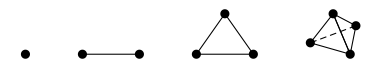
\includegraphics[scale=0.5]{images/simplices.png} }
    \end{center}
    A random variable $X$ with $N+1$ possible values corresponds to a point $x =
    (x_1, \ldots, x_{N+1})$ contained in the simplex $\Delta_N$ in a natural
    way; we set $P[X = i] = x_i$ and equivalently have a probability mass
    function $p(i) = x_i$.
    
    Statisticians are often concerned with families of probability
    distributions.  We identify such families with geometric spaces.
    \begin{definition}
    By the phrase \emph{statistical model}, we mean a subset $\Mod \subset
    \Delta_N$ of a probability simplex.
    \end{definition}
    \noindent A statistical model may be parametrized by a map $f: U \to
    \Delta_N$, for some space $U$ of parameters.
    \begin{example}
        A random variable $X$ following a binomial distribution with size $n$
        and parameter $\lambda \in [0,1]$ takes a value $k \in \{0,\ldots, n\}$
        with probability
        \[
            P_\lambda[X = k] = {n \choose k} \lambda^k(1-\lambda)^{n-k}.
        \]
        This is the number of heads produced by $n$ `coin tosses', where
        $\lambda$ is the probability of a head.  The map $\lambda \mapsto
        P_\lambda$ determines a parametrized statistical model $\{P_\lambda :
        \lambda \in [0,1] \} \subset \Delta_n$. The statistical model is a
        curve, i.e. a one-dimensional subspace, of the simplex.
    \end{example}
    
\subsection{Maximum Likelihood Estimation}

    Given data from an unknown distribution and statistical model $\Mod \subset
    \Delta_N$ of candidate distributions, there is a natural way to select a
    distribution from the model.  We use discrete distributions throughout,
    though these definitions can be made more general.

    Let $\Mod = \{P_\theta : \theta \in U\}$ be a parametrized statistical
    model. A random variable $X$ distributed according to some $P_\theta$ has
    the probability mass function $p_\theta(x) = P_\theta[X = x]$.  Suppose that
    we have some data $Z = \{z_1, \ldots, z_n\}$.  The data are generally assumed to
    be independent and identically distributed according to some unknown true
    distribution in $\Mod$.
    
    \begin{definition}
        The \emph{likelihood function} of $\theta \in U$ given the data $Z$ is
        \[
            L(\theta; Z) = \prod_{i=1}^n p_\theta(z_i).
        \]
        It is the probability that the observed data $Z$ would occur if the
        observations were independent and identically distributed and following
        $P_\theta$.  The \emph{log-likelihood function} is
        \[
            l(\theta; Z) = \sum_{i=1}^n \log p_\theta(z_i)
        \]
        and is often used in place of the likelihood because it is additive.
    \end{definition}
    \begin{definition}
        The \emph{maximum likelihood estimate} of the true parameter is the
        parameter 
        \[
            \mle = \argmax_{\theta \in U} L(\theta; Z)
        \]
        that maximizes the likelihood (or equivalently the log-likelihood) of
        the data.
    \end{definition}

    Notice that the maximum likelihood estimate might not be unique and might
    not even exist.  In practice it is often the case that an exact value for
    $\mle$ is not computed, and instead a good approximation is found via
    numerical techniques.

\subsection{Solutions to the Likelihood Equations}

    Here, we give a flavor of how algebro-geometric techniques can be applied to
    maximum likelihood estimation.  Our exposition follows Section 3.3 of
    \cite{ASCB} and Section 2.1 of \cite{DSS08}.

    Suppose that $g: U \to \Delta_{N-1}$ is a rational parametrization of a
    statistical model, where $U$ is an open subset of $\R^d$.  By rational, we
    mean that each component of $g(\theta) = (g_1(\theta), \ldots, g_N(\theta))$
    is a rational function with rational coefficients in its argument $\theta
    \in U \subset \R^d$.  Maximum likelihood estimation then amounts to
    maximizing the function
    \[
        l(\theta) = \sum_{i=1}^N u_i \log g_i(\theta)
    \] 
    where $u_i$ is the number of times event $i$ has occurred in the observed
    data.

    Every local and global maximum $\theta \in U$ is a solution to the
    likelihood equations
    \begin{equation}\label{eq:lik}
        \frac{\partial l}{\partial\theta_j}
        =
        \sum_{i=1}^N 
        \frac{u_i}{g_i} 
        \cdot
        \frac{\partial g_i}{\partial \theta_j}
        = 0
        \qquad
        \text{for $j = 1,\ldots,d$}.
    \end{equation}
    The likelihood equations in \eqref{eq:lik} are again rational functions of
    $\theta$.  Solving the equations involves `clearing denominators' and
    solving the polynomial equations
    \begin{equation}\label{eq:lik-clear}
        \sum_{i=1}^N 
        u_i \cdot g_1 \cdots \widehat{g_i} \cdots g_N
        \frac{\partial g_i}{\partial \theta_j}
        = 0
        \qquad
        \text{for $j = 1, \ldots, d$}
    \end{equation}
    where $\widehat{g_i}$ indicates that the $i$-th factor is omitted.  The
    equations \eqref{eq:lik-clear}, however, introduce extraneous solutions, for
    example when $g_a(\theta) = g_b(\theta) = 0$ for any $a \ne b$.

    Algebraic geometry offers a principled way to solve the likelihood
    equations.  (For a brief introduction to affine and projective varieties, see
    Appendix \ref{sec:varieties}.)  Consider the ideal $I \subset \R[\theta_1,
    \ldots, \theta_d]$ generated by the polynomial expressions in \eqref{eq:lik-clear}
    \[
        I = \adil[\Bigg]{
            \sum_{i=1}^N u_i \cdot g_1 \cdots \widehat{g_i} \cdots g_N
            \frac{\partial g_i}{\partial \theta_j}
        }_{j=1}^d
        .
    \]
    Let $h$ be the product of all polynomials appearing in the denominators of
    the rational equations in \eqref{eq:lik}.  The \emph{saturation ideal} of
    $I$ with respect to $h$ is defined
    \[
        (I : h^\infty) = \cdil[\big]{
            f \in \R[\theta_1, \ldots, \theta_d]
            \;\big\vert\;
            fh^k \in I
            \quad
            \text{for some non-negative integer $k$}
        }.
    \]
    We can then consider the variety corresponding to the saturation ideal.  The
    points in $V(I : h^\infty) \cap U$ are all solutions to the likelihood
    equations.  In the case that there are only finitely many solutions, passing
    to the saturation ideal removes all extraneous solutions.

    The referenced works \cite{ASCB} and \cite{DSS08} include examples of
    computing the variety $V(I : h^\infty)$ with the software package
    \texttt{Singular}.  An overview of the techniques used to solve such
    polynomial equations, e.g. Gröbner bases, resultants, and elimination, is
    given in the text \cite{CLO05} on computational algebraic geometry.

\subsection{Implicit Models}

    % In the context of algebraic statistics, we usually look at statistical
    % models that are semialgebraic sets.

    % A simplex is the locus of a finite collection of polynomial equations
    % and polynomial inequalities and therefore is a semialgebraic set.


\section{The Restricted Boltzmann Machine}

    We now focus on a statistical model that has recently become important to
    the machine learning community in the pursuit of so-called `deep learning'
    architectures.  In particular, this model is the key component of the `Deep
    Belief Network' which has achieved considerable success at a number of
    machine learning tasks \cite{Hin07}.  For more about the context in which
    the Restricted Boltzmann Machine has become important, see the overview of
    machine learning in Appendix \ref{sec:ML}.

\subsection{The Model}
    \label{sec:rbm-def}

    \begin{definition}
    The \emph{Restricted Boltzmann Machine} (RBM) with $n$ visible units and $k$
    hidden units has binary states of the form $(v, h)$, where $v \in \{0,1\}^n$
    and $h \in \{0,1\}^k$ are binary vectors.  It has real parameters $w_{ij}$,
    $b_i$, and $c_j$, with indices ranging $1 \le i \le n$ and $1 \le j \le k$.
    Its unnormalized joint distribution is
    \begin{equation}\label{eq:rbm-unnorm}
        \psi(v, h) = \exp\pdil*{
            \sum_{ij} w_{ij} v_i h_j + \sum_i b_i v_i + \sum_j c_j h_j
        }
    \end{equation}
    and its actual joint distribution is 
    \[
        p(v, h) = \frac{\psi(v,h)}{Z}
    \] 
    where the normalizing constant $Z = \sum_{v,h} \psi(v, h)$ is the called the
    \emph{partition function}.  The distribution over its visible units is
    \[
        p(v) = \sum_{h \in \{0,1\}^k} p(v,h)
    \]
    a \emph{marginalization} over the hidden states.
    \end{definition}
    The reader familiar with statistical mechanics may recognize this as a
    Boltzmann distribution with energy $H(v,h) = - \log \psi(v, h)$.  The energy
    $H$ is a quadratic polynomial in the visible and hidden variables.  Because
    $H$ contains no terms with two visible or two hidden variables, the RBM is a
    \emph{graphical model} that factors according to the complete bipartite
    graph $K_{n,k}$ on the visible and hidden nodes.
    \begin{center}
    \scalebox{1.0}{ 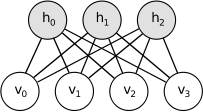
\includegraphics[scale=0.8]{images/rbm.png} }
    \end{center}
    Indeed, if we, for example, take the value $h$ of the hidden units to be
    fixed, then $v \mapsto H(v, h)$ is a linear function and the expression
    $e^{H(v,h)}$ decomposes into a product of functions, each dependent on a
    single component of $v = (v_1, \ldots, v_n)$.  It follows that conditioned
    on a fixed value of $f$, the components $v_i$ are independent random
    variables.  For a description of graphical models in general, refer to
    Appendix \ref{sec:graph}.  A general (as opposed to restricted) Boltzmann
    machine would allow $H$ to be an arbitrary quadratic polynomial, and would
    only factor according to the complete graph on all units.

    
    
\subsection{The Geometry of the Restricted Boltzmann Machine}
    The recent paper \cite{CMS09} examines the Restricted Boltzmann Machine from
    an algebro-geometric perspective.  We outline a small portion of its
    approach.
    
    In the context of algebraic statistics, we want a rational parametrization
    of the model.  To that aim, we replace the parameters $w_{ij}$, $b_i$, and
    $c_j$ used in Section \ref{sec:rbm-def} with
    \[
        \omega_{ij} = \exp(w_{ij})
        \qquad
        \beta_i = \exp(b_i)
        \qquad
        \gamma_j = \exp(c_j)
    \]
    so that $\omega_{ij}$, $\beta_i$, and $\gamma_j$ range over the strictly
    positive real values.  That is, the parameter space is $\R_{>0}^{nk+n+k}$.
    Under this parametrization, the unnormalized probability distribution
    \eqref{eq:rbm-unnorm} becomes
    \[
        \psi(v, h) = 
            \pdil*{ \prod_{i=1}^k \prod_{j=1}^n \omega_{ij}^{h_i v_j} }
            \pdil*{ \prod_{i=1}^n \beta_i^{v_i} }
            \pdil*{ \prod_{j=1}^k \gamma_j^{h_j} }
    \]
    which is a polynomial for any particular value of the binary vectors
    $(v,h)$.  The marginalized distribution over for the visible variables
    factors as
    \[
        p(v) = \frac 1 Z
        \beta_1^{v_1} \beta_2^{v_2} \cdots \beta_n^{v_n} 
        \prod_{i=1}^k
        (1 + \gamma_i \omega_{i1}^{v_1} \omega_{i2}^{v_2} \cdots \omega_{in}^{v_n})
    \]
    where the factors $(1 + \gamma_i \omega_{i1}^{v_1} \omega_{i2}^{v_2} \cdots
    \omega_{in}^{v_n})$ correspond to the choice of whether $h_i = 0$ or $h_i =
    1$.  The partition function $Z = \sum_{v,h} \psi(v,h)$ is also a polynomial
    in the new parameters $\omega$, $\beta$, and $\gamma$,  so the full
    parametrization $\R_{>0}^{nk+n+k} \to \Delta_{2^n-1}$ of the model is a
    rational map.  

    Following \cite{CMS09}, let $M_n^k \subset \Delta_{2^n-1}$ denote the image
    of the parametrization, and let $V_n^k$ denote the Zariski closure of
    $M_n^k$ in the complex projective space $\Proj^{2^n-1}$.  The model $M_n^k$
    is a semialgebraic set.

    In the absence of a `defect', one would expect that both $M_n^k$ and $V_n^k$
    have the same dimension as the parameter space $\R^{nk + n + k}$.  In fact,
    the dimensions are
    \[
        \dim M_n^k = \dim V_n^k = \min\{nk+n+k, 2^n -1\}
    \]
    when $k \le 2^{n - \lceil \log_2(n+1) \rceil}$, which includes most cases of
    practical interest.

    The paper \cite{CMS09} also shows that the varieties $M_n^k$ and $V_n^k$
    `factor'.  Specifically, they factor as \emph{Hadamard powers}
    \[
        V_n^k = (V_n^1)^{[k]}
        \qquad
        M_n^k = (M_n^1)^{[k]}.
    \]
    Then $M_n^1$ and $V_n^1$ are examined.  The variety $V_n^1$ coincides with
    the first secant variety of the \emph{Segre embedding} of the product of
    projective lines $(\Proj^1)^n$ into $\Proj^{2^n-1}$.  The corresponding
    statistical model $M_n^1$ with one hidden value is a mixture of two
    independence models.

    Both the Hadamard product and the Segre embedding are standard
    algebro-geometric constructions.  The Hadamard product $X * Y$ of two
    subvarieties $X$ and $Y$ of a projective space $\Proj^n$ is defined to be
    the Zariski closure of the image of the rational map
    \[
        X \times Y \dashrightarrow \Proj^m,
        \quad
        (x, y) \mapsto [x_0y_0: x_1y_1 : \cdots : x_n y_n].
    \]
    The Segre embedding of the cartesian product of two subvarieties $X \subset
    \Proj^m$ and $Y \subset \Proj^n$ is the image of the map
    \[
        X \times Y \to \Proj^{(m+1)(n+1) - 1},
        \quad
        (x, y) \mapsto
        [x_0y_0: x_0 y_0 : \cdots : x_my_n]
    \]
    where the indices are in lexicographic order.

    Viewing the RBM as an `inference function' from hidden values to the more
    likely visible values, the components $v_i$ of $v$ are
    `linear threshold functions' of $h$.  That is, the values of $h$ are
    vertices of a hypercube, and the decision boundary of whether $v_i = 0$ or
    $1$ is a linear hyperplane through the hypercube.

\subsection{The Nested Sequence}

\subsection{Known Results: Dimensionality and Universal Approximators}

\subsection{Open Questions}


\section{The Hadamard Product}
    

\section{Binary Independence Models}


\subsection{The Independence Model}
    Independence conditions arise naturally in many statistical questions.
    Essentially, they allow portions of a model to be considered separately.

    First, we introduce some notation.  For any positive integer $m$, let $[m] =
    \{1, 2, \ldots, m\}$; this is used when we need a finite set with $m$
    elements.

    Suppose that the random variables $X$ and $Y$ have state spaces $[r]$ and
    $[c]$, respectively.  By definition, $X$ and $Y$ are independent if their
    joint distribution over $[r] \times [c]$ factors into a distribution over
    $[m]$ and another over $[n]$.  
    
    Then the independence model $\Mod \subset \Delta_{rc - 1}$ is the space of
    distributions of the form
    \[
        P(X = i, Y = j) = p_i q_j
        \qquad
        \text{where $p \in \Delta_{m-1}$ and $q \in \Delta_{n-1}$}.
    \]
    \begin{example}
    If $r = c = 2$ (i.e. if $X$ and $Y$ are binary) then the possible
    distributions look like
    \begin{center}
    \begin{tabular}{l|cc}
    & $X = 1$ & $X = 2$\\
    \hline
    $Y = 1$ & $\alpha\beta$ & $(1-\alpha)\beta$\\
    $Y = 2$ & $\alpha(1-\beta)$ & $(1-\alpha)(1-\beta)$
    \end{tabular}
    \end{center}
    for some $\alpha, \beta \in [0,1]$.  
    \end{example}

    Another way to view the independence model is as the set of all $r\times c$
    matrices of rank 1 with non-negative entries that sum to 1.  For a matrix of
    rank 1, all rows (and columns) are multiples of each other, so the rank 1
    condition is equivalent to the condition that the distribution factors.
    
    The independence model has the parametrization
    \begin{IEEEeqnarray*}{rCrCl}
        \phi &:& \Delta_{m-1} \times \Delta_{n-1} &\to& \Mod \subset \Delta_{rc-1}\\
        && \phi_{ij}(p, q) &=& p_i q_j.
    \end{IEEEeqnarray*}
    The model $\Mod$ also has an implicit description.  The points in the variety
    \[
        V = \cdil[\big]{
        \phi \in \R^{rc} 
        \vbar
        \phi_{ij} - (\phi_{i+})(\phi_{+j}) = 0
        \quad
        \text{for all $i \in [m]$ and $j \in [n]$}
        }
    \]
    satisfy the independence condition because the probability $\phi_{ij}$ that
    $(i,j)$ occurs must factor into the probability $\phi_{i+}$ that $i$ occurs
    and the probability $\phi_{+j}$ that $j$ occurs.  The independence model is
    then the intersection $\Mod = V \cap \Delta_{rc-1}$, and is clearly a
    semialgebraic set.

\subsection{Hidden Variables and Mixture Models}
    Consider a random variable $X$ with state space $[r]$, and suppose that
    another random variable $Y$ with state space $[c]$ has an influence on $X$.
    If $Y$ has some prior distribution $\pi$, then the joint distribution of $X$
    and $Y$ is 
    \[
        P(X = i, Y = j) = \pi_j \cdot p_i^{(j)}
    \]
    where $\{p^{(j)} \mid j \in [c]\}$ is some collection of distributions.

    If $Y$ is a hidden variable, we can only observe the marginal distribution
    of $X$.  The marginal probability is the sum over the possible hidden values
    \[
        P(X = i) = \sum_{j \in [c]} \pi_j \cdot p_i^{(j)}.
    \]
    A hidden variable model allows for the creation of a potentially more
    complex model out of simple components $p^{(j)} \in \Delta_{r-1}$.
    In particular, if the distributions $p^{(j)}$ are required to lie in some
    model $V \subset \Delta_{r-1}$, then we have a mixture model.
    \begin{definition}
    Suppose that $V$ and $W$ are subsets of the affine space $\R^n$.  Their
    \emph{mixture} is the set
    \[
        \Mixt(V, W) = \cdil[\big]{
        \lambda v + (1 - \lambda)w \vbar
        v \in V, w \in W, \lambda \in [0,1]
        }.
    \]
    A mixture of $V$ with itself $k$ times produces the higher mixture
    \[
        \Mixt^k(V) = \cdil*{
        \sum_{i=1}^k \lambda_i v_i \vbar v_i \in V, \lambda_i \in [0,1],
        \text{and }\lambda_1 + \cdots \lambda_s = 1
        }.
    \]
    A \emph{mixture model} is a statistical model produced by mixtures.
    \end{definition}

    \begin{example}
    A \emph{Gaussian mixture model} is a simple model that is useful in a wide
    variety of situations.  A Gaussian distribution with parameters $(\mu,
    \sigma)$ has probability density
    \[
        p_{\mu, \sigma}(x) = \frac{1}{\sqrt{2\pi\sigma^2}} 
        \exp\pdil*{-\frac{(x - \mu)^2}{2\sigma^2}}.
    \]
    A mixture of two Gaussian distributions is a weighted sum $p(x) = \lambda
    p_{\mu_1, \sigma_1}(x) + (1 - \lambda)p_{\mu_2, \sigma_2}(x)$.  
    \begin{center}
    \scalebox{1}{ 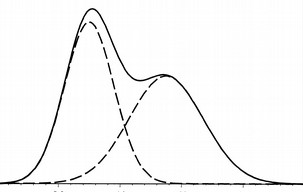
\includegraphics[scale=0.5]{images/mixture.png} }
    \end{center}
    (The space of distributions over the real line is not finite dimensional,
    but in this case works similarly.) Mixtures of more or higher dimensional
    Gaussian distriubtions are defined as one would expect.  Such models are
    useful, for instance, for clustering tasks.
    \end{example}

    Mixture models correspond to a relatively well-studied object in algebraic
    geometry.
    \begin{definition}
    The \emph{secant variety} of the affine variety $V \subset \F^n$ is
    \[
        \Sec(V) = \overline{\cdil[\big]{
        \lambda u + (1 - \lambda) v \vbar
        u,v \in V
        \text{ and }
        \lambda \in \F
        }}
    \]
    where the line indicates the Zariski closure of the set.  Higher secant
    varieties are defined in the natural way, that is, $\Sec^1(V) = V$ and
    $\Sec^k(V) = \Sec(Sec^{k-1}(V), V)$ for $k \ge 2$.
    \end{definition}

    There is a reasonably straightforward relationship between mixture models
    and secant varieties.
    \begin{proposition}[\cite{DSS08}]
    If $V$ is a semialgebraic set, then the secant variety
    $\Sec^k(\overline{V})$ is the Zariski closure of the mixture $\Mixt^k(V)$.
    \end{proposition}

\section{Steps Forward}

\begin{comment}
    The marginal distribution of the RBM over its visible variables is
    \[
        p_V(v) = \sum_{h \in \{0,1\}^k} p(v, h).
    \]
    Given a fixed value $h$ for the hidden variables, the visible variables are
    all independent.  It follows that the marginal distribution over the visible
    variables is a mixture of independence models.  The mixture model can have
    up to $2^k$ components, because there are $2^k$ possible states for the
    hidden variables.

    In some sense, the hidden variables constitute an `explanation' for the
    observed variables.  That is, a particular value of $v$ induces a
    probability distribution over possible values $h$ of the hidden variables.
    This observation motivates a number of uses for the RBM, including as the
    building block for the Deep Belief Network, discussed later.
\end{comment}




\appendix

\section{A Little Algebraic Geometry}

    The field of algebraic geometry grew out of the study of curves and surfaces
    determined by polynomials.  In the mid-twentieth century, the foundations of
    the subject were reformulated by Serre, Grothendieck, and others.  The
    techniques of the field are notoriously both abstract and powerful; the
    following quote by the algebraic geometer David Mumford is perhaps telling
    \cite{Mum99}.
    \begin{quote}
        Algebraic geometry seems to have acquired the reputation of being
        esoteric, exclusive, and very abstract, with adherents who are secretly
        plotting to take over all the rest of mathematics.  In one respect this
        last point is accurate.
    \end{quote}
    More recently, the development of algorithmic techniques, e.g. Gröbner
    bases, has spurred interest in the field of computational algebraic
    geometry.  A standard introduction to algebraic geometry from a
    computational perspective is \cite{CLO97}, which covers algebraic varieties
    and Gröbner bases algorithms while assuming a relatively small amount of
    prerequisite knowledge.  The same authors have a graduate text \cite{CLO05}.

    Here, we introduce some classical algebro-geometric objects.  There are many
    references in which these objects and their importance is explicated; one is
    \cite{Sha}.

\subsection{Affine and Projective Varieties}
    \label{sec:varieties}
    Throughout, let $\F$ be a field.  It is useful to think of $\F$ being either
    $\R$ or $\C$.

    Let $\A^n$ be the affine space of dimension $n$ over $\F$ (that is, the
    vector space $\F^n$ where we view neither the choice of basis nor the choice
    of origin as canonical).  A polynomial $f \in \F[x_1, \ldots, x_n]$ can be
    considered as a function on $\A^n$ by simply evaluating the polynomial on
    any given point.

    \begin{definition}
        An \emph{affine algebraic set} is a subset of the affine space $\A^n$
        of the form
        \[
            V(f_1, \ldots, f_m)
            = \cdil[\big]{x \in \A^n \vbar f_i(x) = 0 \quad\text{for all $i$}}
        \]
        for some finite set of polynomials $f_i \in \F[x_1, \ldots, x_n]$.
    \end{definition}
    \noindent Instead of a finite set of polynomials, we can equivalently
    consider a finitely generated ideal.  In fact, $\F[x_1,\ldots,x_n]$ is a
    Noetherian ring, so the condition that the ideal be finitely generated
    condition is redundant.

    Given a subset $X \subset \A^n$, we may consider the ideal of polynomials
    vanishing on the subset
    \[
        I(X) = \cdil[\big]{f \in \F[x_1, \ldots, x_n] \vbar f(x) = 0 \quad\text{for
        all $x \in X$}}.
    \]
    Under certain conditions (e.g. if the field is algebraically closed and the
    ideal is \emph{radical}), the operations $V$ and $I$ are inverses of each other.

    \begin{definition}
        The \emph{projective space} of dimension $n$ (usually denoted $\Proj^n$)
        is the space $\F^{n+1}\setminus \{0\}$ under the equivalence relation $x
        \sim \lambda x$ for $x \in \F^{n+1}$ and $0 \ne \lambda \in \F$.  The
        usual affine coordinate system on $\F^{n+1}$ modulo scaling gives
        \emph{homogeneous coordinates} $[x_0: \cdots: x_n]$ on $\Proj^n$.  If
        $\F = \R$ (resp.  $\C$), the homogeneous coordinates give $\Proj^n$ the
        structure of a real (resp. complex) manifold.
    \end{definition}

    It also turns out that projective space behaves particularly nicely for the
    purposes of algebraic geometry, for reasons that we will not describe here.
    Instead of arbitrary polynomials, a different collection of `functions' is
    used on projective space.
    \begin{definition}
        A \emph{homogeneous polynomial} in $n+1$ variables of degree $d$ is a
        polynomial of the form $F(x) = \sum a_I x^I$ where $a_I \in \F$ and the
        multi-index ranges over $I = (i_0, \ldots, i_n)$ such that $i_0 + \cdots
        + i_n = d$.  The monomials are defined to be $x^I = x_0^{i_0}\cdots
        x_n^{i_n}$.  A \emph{homogeneous ideal} is an ideal of $\F[x_0, \ldots,
        x_n]$ generated by homogeneous polynomials.
    \end{definition}
    Notice that if $F$ is homogeneous polynomial of degree $d$, then $F(\lambda
    x) = \lambda^d F(x)$ for $\lambda \in \F$.  The zero set of $F$ in $\Proj^n$
    is then well-defined.  It follows that we can define the projective analogue
    of an affine variety.
    \begin{definition}
        A \emph{projective variety} is a subset of the projective space
        $\Proj^n$ of the form
        \[
            V(f_1, \ldots, f_m)
            = \cdil[\big]{x \in \Proj^n \vbar f_i(x) = 0 \quad\text{for all $i$}}
        \]
        for some finite set of homogeneous polynomials $f_i \in \F[x_0,
        \ldots,x_n]$.
    \end{definition}
    As in the affine case, there is a well-behaved correspondence between the
    homogeneous ideals of $\F[x_0, \ldots, x_n]$ and projective varieties.

    Using these varieties, we may define the \emph{Zariski topology} on $\A^n$
    and $\Proj^n$;  the affine (or projective) varieties are the closed sets of
    the topology.  The Zariski topology is a bit unusual as, unless the field is
    finite, no variety is ever a Hausdorff space.

    For the applications encountered in algebraic statistics, we will need to
    venture into real algebraic geometry, the primary objects of which are
    slightly less well-behaved.
    \begin{definition}
        A \emph{semialgebraic set} is any subset of $\R^n$ of the form
        \[
            V = \cdil[\big]{ x \in \R^n \vbar
                f_i(x) = 0, g_j(x) > 0
            \quad\text{for all $i,j$}}
        \]
        for some finite collection of polynomials $f_i, g_j \in \R[x_1, \ldots,
        x_n]$.
    \end{definition}

    A more in-depth investigation into algebraic geometry reveals the central
    importance of rings of functions on spaces, and the need to consider
    arbitrary commutative rings.  This road leads to the theory of schemes,
    which we will neither need nor pursue here.

\section{Machine Learning: Goals, Techniques, and Trends}
    \label{sec:ML}

    The goal of machine learning is to algorithmically use data in order to
    perform specified tasks better.  The emphasis of the field, tends to be
    toward large data sets, efficient algorithms, and `non-parametric' models
    with few assumptions.  Machine learning is studied both by computer
    scientists and statisticians.  The text \cite{ESL} is an excellent overview
    of machine learning from the latter perspective.

\subsection{Statistical Classification}

    One common task is the classification problem.  Here, observations are
    points in some usually large, complicated, or high-dimensional space $X$,
    and the task is to assign a class label to an observation $x \in X$.  Class
    labels come from finite set $C$, and usually have some meaning.
    Classification can also be viewed as an attempt to approximate a function $f
    : X \to C$ given a training data set $\{(x_i, f(x_i)\}_{i=1}^n$ of
    observations.  Of course for this task to be feasible, there must be strong
    constraints on the functions under consideration; we must select a model.

    \begin{example} 
    One dataset commonly seen in the literature is the MNIST dataset of
    handwritten digits \cite{MNIST}.
    \begin{center}
    \scalebox{0.8}{
    
\includegraphics{images/mnist_0.png}\,
    
\includegraphics{images/mnist_1.png}\,
    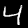
\includegraphics{images/mnist_2.png}\,
    
\includegraphics{images/mnist_3.png}\,
    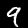
\includegraphics{images/mnist_4.png}
    }
    \end{center}
    Each $28\times28$ pixel image depicts a handwritten digit.  The training set
    contains 60,000 examples and the test set contains 10,000 examples.  The
    task is to classify each image in the test set as one of the digits
    $0,1,\ldots,9$.
    \end{example}

    The majority of successful algorithms are in some sense `only a step or two
    away from linear'.  For instance the \emph{perceptron}, a binary linear
    classifier, places observations (which are real vectors) into two classes by
    learning a hyperplane which separates the classes.  The \emph{support vector
    machine} takes a modified approach, as it maps the observed data to a very
    high-dimensional space, and learns a separating hyperplane there.  Another
    common approach is to construct an approximating function as a weighted
    linear combination of a family of basis functions.

    For some problems, however, these techniques may not be sufficient.  Within
    the past ten years, there has been increased interest in so-called `deep
    learning' methods.  An overview of the motivating problems of deep learning
    is contained in \cite{Ben09}.  Perhaps the most influential technique put
    forward so far is the Deep Belief Network.


\subsection{The Deep Belief Network}
    A Deep Belief Network (DBN) is a generative model consisting essentially a
    stack of RBMs, trained greedily.  The paper \cite{Hin07} introduced a
    technique known as `contrastive divergence' that allowed RBMs, and in turn
    DBNs, to be trained efficiently on problems of practical interest.
    \begin{definition}
    A \emph{Deep Belief Network} is a model on multiple layers of hidden
    variables, built out of RBMs.  Specifically, let $h^k \in \{0,1\}^{n_k}$
    denote the binary state vector of the $k^{\text{th}}$ layer for $0 \le k \le
    m$.  The layer $h^0$ is the visible layer.  The joint distribution of the
    DBN is
    \begin{align*}
        P(v,h^1, \ldots, h^m) &= P(h^{m-1}, h^m) \prod_{k=0}^{m-2} P(h^k \mid h^{k+1})\\
        P(h^k\mid h^{k+1}) &\propto \exp\pdil*{(h^k)^Tb^k + (h^k)^T W^{k+1} h^{k+1}}\\
        P(h^{m-1}, h^{m}) &\propto  \exp\pdil*{(h^{m-1})^T b^k + (h^{m-1})^T W^m
        h^m + (h^m)^T b^m}
    \end{align*}
    for some collection of parameters $b^k$ and $W^k$.
    \end{definition}

    The conditional independence structure of the DBN is described by a graph
    with undirected connections between the top two layers and directed
    connections between all other adjacent layers.
    \begin{center}
    \scalebox{0.6}{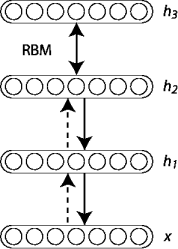
\includegraphics{images/DBN3.png}}
    \end{center}
    For classification, the network would be greedily trained to represent the
    input data.  The top layer $h^m$ would then be trained to classify the
    inputs with a one-hot encoding.

\subsection{Graphical models}
    \label{sec:graph}

    A graphical model is a probabilistic model for which a graph (directed or
    undirected) represents the conditional independence structure between random
    variables. 

    Let $G$ be a graph with vertex set $V$.  Suppose that $(X_\alpha)_{\alpha
    \in V}$ are random variables.  It is common for the $X_\alpha$ to be either
    discrete or real-valued.  The joint probability of $X = (X_\alpha)$ is said
    to factor with respect to $G$ if the probability density is
    \[
        p(X_1, \ldots, X_n) = 
            \prod_\alpha p(X_\alpha \mid X_\beta, \beta \text{ is a parent of }
            \alpha).
    \]
    The dependence of a random variable on the other variables is completely
    captured by its dependence on its immediate parents (i.e. on the variables
    having directed edges into it).  It is also possible to formulate an
    equivalent statement in terms of conditional independence statements.

    In the case of an undirected graph, it is known (in a result called the
    Hammersley–Clifford theorem) that the probability density factors as
    \[
        p(X_1, \ldots, X_n) = 
            \prod_{S \in C(G)} p(X_\alpha \mid X_\beta, \beta \in S)
    \]
    where the $S$ are complete subgraphs (cliques) of $G$.

    Graphical models turn up in a number of places: Bayesian networks (directed)
    and Markov random fields (undirected) in statistics, Boltzmann machines in
    machine learning, and Ising models (particle spins in a lattice) in
    statistical mechanics.

\nocite{*}
\bibliographystyle{annotate}
\bibliography{mid}

\begin{comment}
\begin{thebibliography}{100}
    \bibitem[BCR98]{BCR98} Bochnak, Coste, Roy.  Real Algebraic Geometry.  1998.
    \bibitem[Ben09]{Ben09} Bengio.  Learning Deep Architectures for AI. 2009.
    \bibitem[CLO92]{CLO92} Cox, Little, O'Shea.  Ideals, Varieties, and
    Algorithms.  1992.
    \bibitem[CLO98]{CLO98} Cox, Little, O'Shea.  Using Algebraic Geometry.  1998.
    \bibitem[CLS09]{CLS09} Cox, Little, Schenck.  Toric Varieties.  2009.
    \bibitem[CMS09]{CMS09} Cueto, Morton, Sturmfels. Geometry of the Restricted Boltzmann Machine.  2009.
    \bibitem[Cos09]{Cos09} Michel Coste.  An Introduction to Semialgebraic Geometry.  2002.
    \bibitem[CTY10]{CTY10} Cueto, Tobis, Yu.  An Implicitization Challenge for Binary Factor Analysis. 
    2010.
    \bibitem[DS98]{DS98} Diaconis and Sturmfels.  Algebraic Algorithms for Sampling
    from Conditional Distributions. 1998.
    \bibitem[DSS08]{DSS08} Drton, Sturmfels, Sullivant. Lectures on Algebraic
    Statistics. 2009.
    \bibitem[GMS06]{GMS06} Geiger, Meed, Sturmfels.  On the Toric Algebra of Graphical Models. 2006.
    \bibitem[Hin07]{Hin07} Hinton.  A Fast Algorithm for Deep Belief Nets.  2007.
    \bibitem[MA10]{MA10} Montufar, Ay.  Refinements of Universal Approximation
    Results for Deep Belief Networks and Restricted Boltzmann Machines.  2010.
    \bibitem[Mon10]{Mon10} Montufar.  Mixture Models and Representational Power of
    RBM's, DBN's and DBM's.  2010.
    \bibitem[PS03]{PS03} Pachter, Sturmfels.  Tropical Geometry of Statistical Models. 2003.
    \bibitem[Ric09]{Ric09} Riccomagno.  A Short History of Algebraic Statistics.  2009.
    \bibitem[Top02]{Top02} Topics in Algebraic Geometry and Geometric Modeling:
    Workshop on Algebraic Geometry and Geometric Modeling July 29 -- August 2,
    2002 (Contemporary Mathematics).  Ed. by Goldman and Krasauskas.
    \bibitem[Wat09]{Wat09} Watanabe.  Algebraic Geometry and Statistical Learning Theory.  2009.

    \bibitem{A5} Pachter, Sturmfels.  ``Tropical Geometry of Statistical
    Models''. 2003.
    \bibitem{A6} Pachter, Sturmfels.  \textit{Algebraic Statistics for
    Computational Biology}.  2005.
\end{thebibliography}
\end{comment}


\end{document}
